
\documentclass[11pt]{article}

\usepackage{times}

\usepackage{epsfig}		% EPS figures
\usepackage{subfig}		% subfigures
\usepackage{float}		% floating objects
\usepackage{verbatim}	% allows multi-line comments

\usepackage{setspace}	% For 2x spacing
%\doublespacing
\onehalfspacing
% If double-spacing is too much...
%From the setspace.sty: for 11pt font,
% \doublespacing == \setstretch{1.618}
% \onehalfspacing == \setstretch{1.213}
%\setstretch{1.32} 

% Math! In case we need it
%\usepackage{amsmath}
%\usepackage{amsfonts}
%\usepackage{amssymb}
%\usepackage{graphicx}

% For headers
\usepackage{fancyhdr}
\usepackage{datetime}

% For list spacing, see below
\usepackage{atbeginend}

%For fancy tables
\usepackage{multirow}

%Good url formatting in bibliography
\usepackage{url}

% 1 inch on each side for A4 printing
\setlength{\textwidth}{6.5in}
\setlength{\textheight}{9in}

%If dvipdf is used
%\setlength{\topmargin}{0.65in}

%If pdfetex is used
\setlength{\topmargin}{-0.1in}

\setlength{\oddsidemargin}{0.0in}
%\setlength{\oddsidemargin}{-0.125in}
%\setlength{\oddsidemargin}{-0.25in}
%% \setlength{\evensidemargin}{-0.25in}
\setlength{\parindent}{0.4in}
\setlength{\parskip}{0.05in}
\addtolength{\topmargin}{-0.5in}

%Let's squeeze things a bit, as with double spacing some separations are just ridiculous
%\addtolength{\intextsep}{-0.06in}
\addtolength{\floatsep}{-0.06in}
\addtolength{\textfloatsep}{-0.04in}
\addtolength{\abovecaptionskip}{-0.03in}
\addtolength{\belowcaptionskip}{-0.03in}
% For lists
%\addtolength{\topsep}{-0.2in}
%\addtolength{\partopsep}{-0.2in}
%\addtolength{\itemsep}{-0.05in}

\AfterBegin{itemize}{\addtolength{\topsep}{-0.1in}}
\AfterBegin{itemize}{\addtolength{\partopsep}{-0.1in}}
\AfterBegin{itemize}{\addtolength{\itemsep}{-0.1in}}

\AfterBegin{enumerate}{\addtolength{\topsep}{-0.1in}}
\AfterBegin{enumerate}{\addtolength{\partopsep}{-0.1in}}
\AfterBegin{enumerate}{\addtolength{\itemsep}{-0.1in}}

%\setlength{\topsep}{0in}
%\setlength{\partopsep}{0in}
%\setlength{\itemsep}{0in}

\newcommand{\icolwidth}{20pc}
\newcommand{\hzline}{\makebox[\icolwidth]{\hrulefill}}
\newcommand{\widehzline}{\makebox[\textwidth]{\hrulefill}}


% Alter some LaTeX defaults for better treatment of figures:
    % See p.105 of "TeX Unbound" for suggested values.
    % See pp. 199-200 of Lamport's "LaTeX" book for details.
    %   General parameters, for ALL pages:
    \renewcommand{\topfraction}{0.9}	% max fraction of floats at top
    \renewcommand{\bottomfraction}{0.8}	% max fraction of floats at bottom
    %   Parameters for TEXT pages (not float pages):
    \setcounter{topnumber}{2}
    \setcounter{bottomnumber}{2}
    \setcounter{totalnumber}{4}     % 2 may work better
    \setcounter{dbltopnumber}{2}    % for 2-column pages
    \renewcommand{\dbltopfraction}{0.9}	% fit big float above 2-col. text
    \renewcommand{\textfraction}{0.07}	% allow minimal text w. figs
    %   Parameters for FLOAT pages (not text pages):
    \renewcommand{\floatpagefraction}{0.7}	% require fuller float pages
	% N.B.: floatpagefraction MUST be less than topfraction !!
    \renewcommand{\dblfloatpagefraction}{0.7}	% require fuller float pages


% Temporary macros. Move out for submission-ready version!
%\newcommand{\note}[1]{{\bf [~NOTE:~#1~]}}
%\newcommand{\fixme}[1]{{\bf [~FIXME:~#1~]}}
%\newcommand{\todo}[1]{{\bf [~TODO:~#1~]}}

\usepackage{color}
\newcommand{\tmp}[1]{{\textcolor{red}{#1~}}}


% Headers -- uncomment for submission
%\date{}
%\pagestyle{plain}

%% Headers -- comment these for submission
%\pagestyle{fancyplain}
%\fancyhf{}
%\renewcommand{\headrulewidth}{0.0pt}
%\chead{\textbf{DRAFT --- \today \hspace*{0.1cm}  \currenttime}}
%\cfoot{\thepage}


\title{A Novel Architecture for Gene Sequence Alignment}
\author{Albert Ng, Sam D'Amico, Asif Khan\\ \emph{\{albertng, sdamico, asifk\}@stanford.edu}}
\date{}

\begin{document}


\maketitle

% In a blind submission you probably want to cover up the space for the authors
%\vspace{-0.6in}
\begin{abstract}

%If using multiple files
%\input{0_abstract.tex}

Whole human genome sequencing costs are projected to fall below \$1000 in the near future, causing an expected skyrocketing in demand for individual genome sequencing.  The short read alignment step of the sequencing process currently takes on the order of a CPU day to complete with state-of-the-art software.  To address this computational bottleneck, hardware accelerators have been implemented, but have only been able to achieve moderate performance improvements.  We perform a case study on an example exact alignment algorithm to understand the performance bottlenecks of both software and hardware implementations.  We conclude that hardware acceleration is memory bandwidth limited, and future accelerator architectures should focus on cost-effective ways to increase memory bandwidth as opposed to more processing power. 

\end{abstract}

% If using multiple files
%\input{1_introduction.tex}
%\input{2_background.tex}
% ...

\section{Introduction}
\par
Modern genetic research has found an increasing number of links between many diseases and one's DNA.  These important discoveries have sparked a large interest in high throughput gene sequencing techniques in recent years, in the hopes of developing medicine that can be personalized to the patient.  National Human Genome Research Institute data shows that as next generation sequencing processes are developed, the cost of sequencing a human genome has been rapidly decreasing, even faster than Moore's Law-like rates \cite{wetterstrand2011dna}.  It is projected that the cost of sequencing a single genome will reach as low as \$1000 in the next few years - well within the average family's medical budget.  With the prospective benefits of knowing one's genome, the demand for gene sequencing is expected to skyrocket in the near future.


High throughput gene sequencing techniques typically involve splitting DNA strands into many small fragments.  These small fragments are sequenced in parallel using chemical and optical techniques, and produce short reads.  To reconstruct the original DNA sequence, the process takes advantage of the fact that over 99\% of human genomes are identical.  Instead of reconstructing the sequence from scratch, as in \textit{de novo} assembly, the short reads are aligned to a reference human genome using inexact alignment algorithms to identify the points of mutations.  A human genome consists of over 3 billion base pairs, and the short reads produced by current sequencing machines are around 100 base pairs long.  Accounting for a typical 10-30x coverage, the number of short read alignments to be performed for a single human genome is in the hundreds of millions.  Thus, this sequence alignment step is very computationally expensive.


	Much research effort has been put towards developing optimized sequence alignment algorithms over the past few decades \cite{smith1981textordfeminineidentification, altschul1990basic, ning2001ssaha, toh2009basic, zaharia2011faster, li2009fast}.  These algorithms typically make tradeoffs between runtime, memory requirement, and alignment accuracy.  Current state-of-the-art algorithms require about a CPU day to align the short reads for a single human genome with acceptable accuracy.  Considering a world population in the billions, these runtimes are not scalable.


To address this issue, efforts have since focused on efficient GPU and FPGA implementations for performance improvement \cite{klus2012barracuda, liu2012soap3, okawa2012pico}.  However, the required design expertise and cost to performance ratio have not been very attractive.  For example, the SOAP3 GPU implementation manages to achieve only a 22x improvement in performance over a single CPU core implementation, despite the hundreds of threads available in the GPU.  Furthermore, the Pico Computing FPGA implementation of BWA yields a 48x speedup over a single core CPU, but utilizing 12 Kintex-7 FPGAs at a system cost of many tens of thousands of dollars.


The goal of this project is to understand the bottlenecks of these accelerators by performing a case study on an example algorithm.  For simplicity, we explore an exact alignment algorithm that uses techniques typically incorporated within modern inexact alignment algorithms.  First, we study a single threaded software implementation of the algorithm to understand its properties and tradeoffs.  We then build a cycle-accurate simulator of a hardware accelerator implementation.  Finally, we study the properties and tradeoffs of this hardware architecture using the simulator.

\section{Alignment Algorithm}

The alignment algorithm is based on the premise that we can split a given search query into a set of smaller subreads each of length $k$. Then, for every possible subread of length $k$ we can store a list of positions in the reference genome where the subread is found. We then flatten this list into an array to create a position table. Because each given subread has a variable number of locations where it is found in the reference genome, we also create another auxiliary interval table which gives us the indices within the position table for that subread. Thus, the search is performed by looking up a list of positions for each subread, and then stitching together the common locations between the different subread locations to determine a list of positions for the longer search sequence.  This is illustrated in Figures \ref{archprocess} and \ref{algorithm}.
\begin{figure}[ht!]
\centering
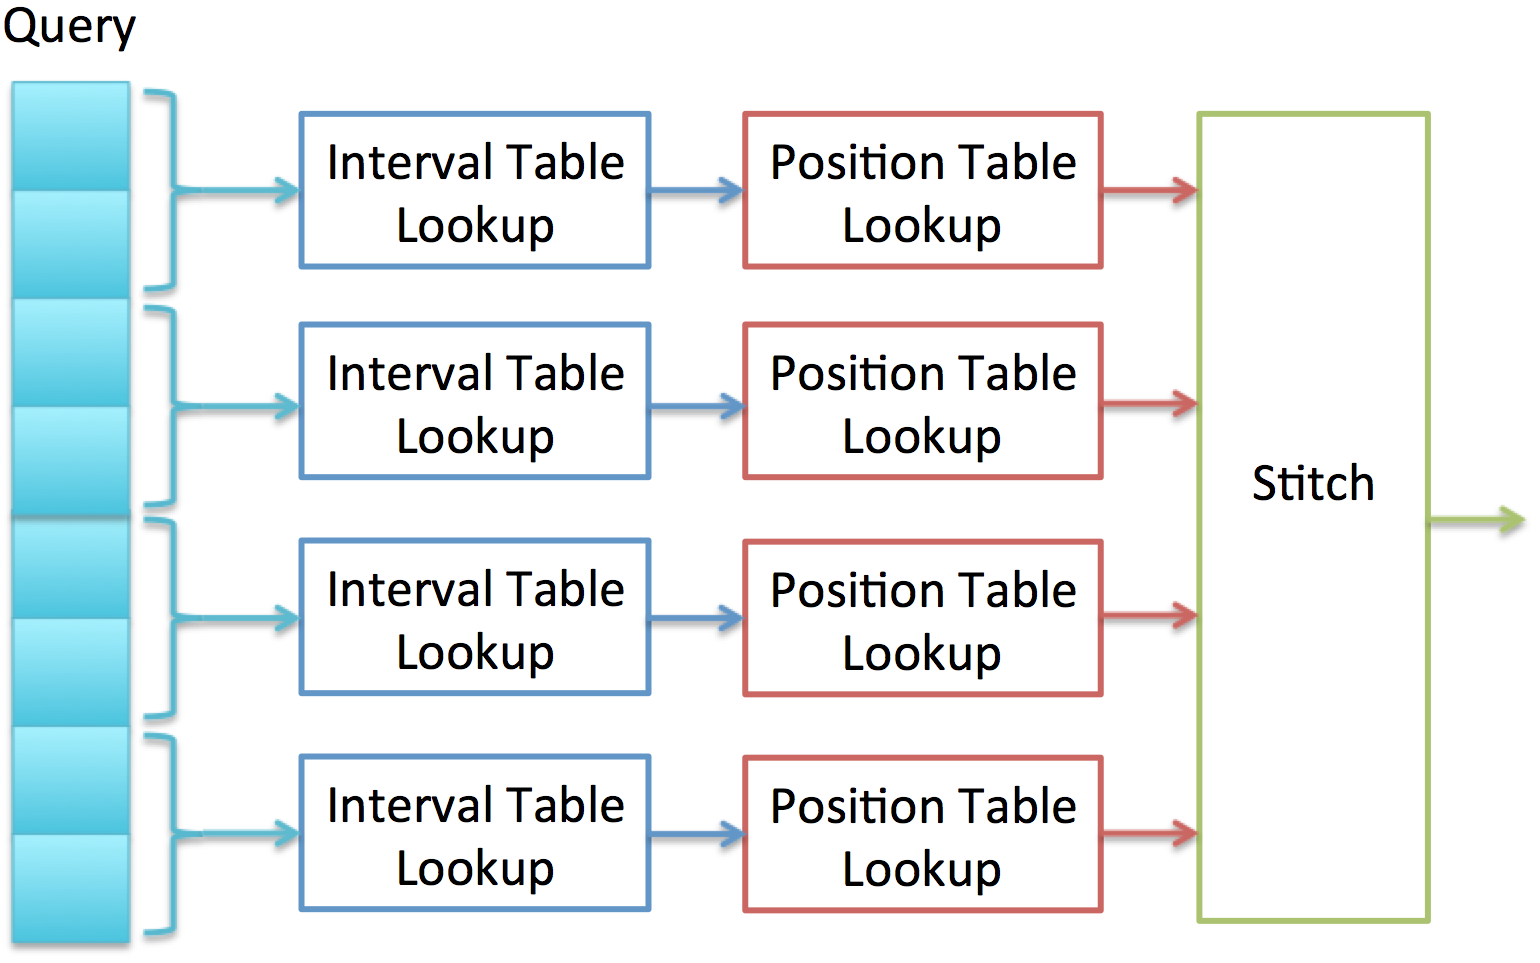
\includegraphics[width=90mm]{archprocess.png}
\caption{Algorithm Overview}
\label{archprocess}
\end{figure}

\begin{figure}[ht!]
\centering
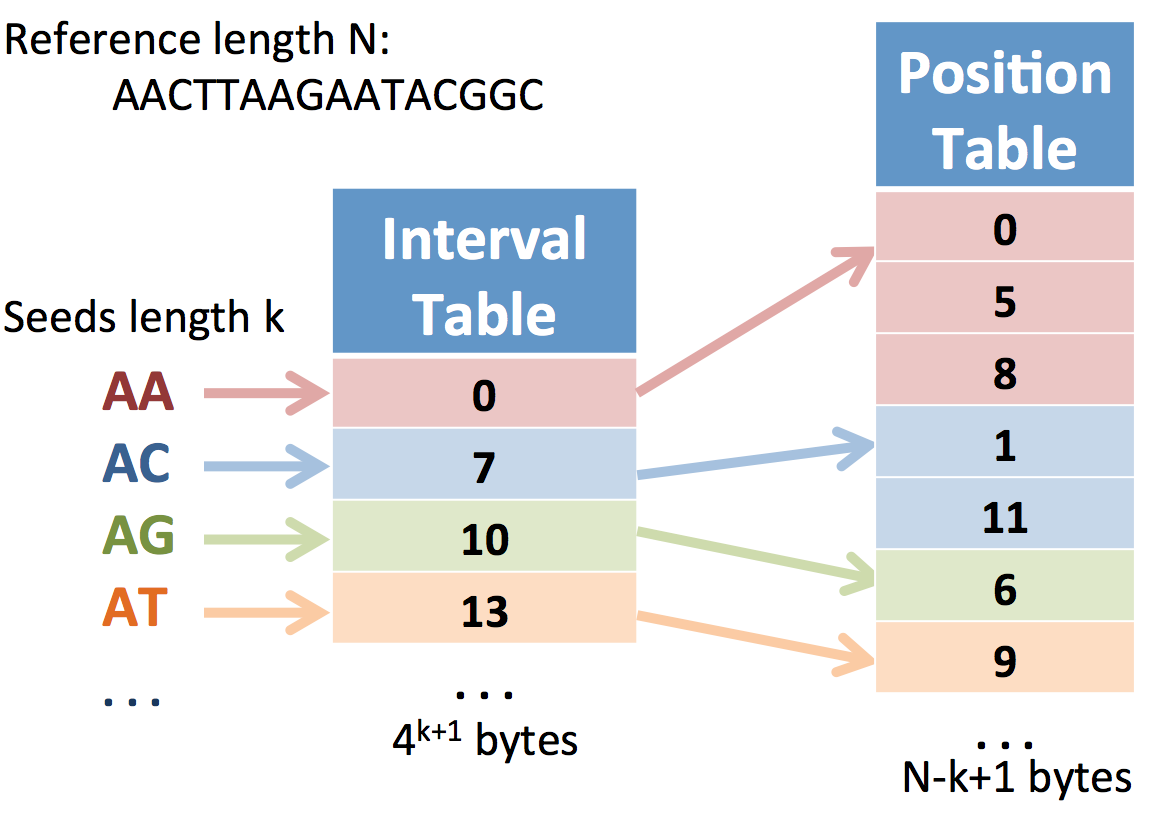
\includegraphics[width=90mm]{algorithm.png}
\caption{Data Structure Accesses}
\label{algorithm}
\end{figure}


The memory requirements for this algorithm for subreads of length $k$ and a reference genome of length $N$ requires $4^k$ entries in the interval table and $N-k+1$ entries in the position table. Each entry is an index into the reference genome, and so each entry requires $\log_2 N$ bits.

\section{Software Simulation}

In order to gain some intuition about the algorithm, we first developed a software implementation and ran it on a machine with a dual quad-core Intel Xeon E5520 @ 2.27GHz and 12 GB RAM for 1,000,000 reads of length 100 (typical for most sequencing hardware) on a reference human chromosome of 225 million nucleotides.


As seen in Figure \ref{speedvsseedlen}, we notice that the speed decreases sharply as we increase the seed length. This makes sense intuitively - for short subreads, the position table entries are much longer and thus there are both more memory reads required and more computation needed for the stitching algorithm.  Figure \ref{histogram} helps to illustrate how the average position table list length varies with seed length. The tradeoff with increasing the seed length, however, is that our interval table size grows exponentially.
\begin{figure}[ht!]
\centering
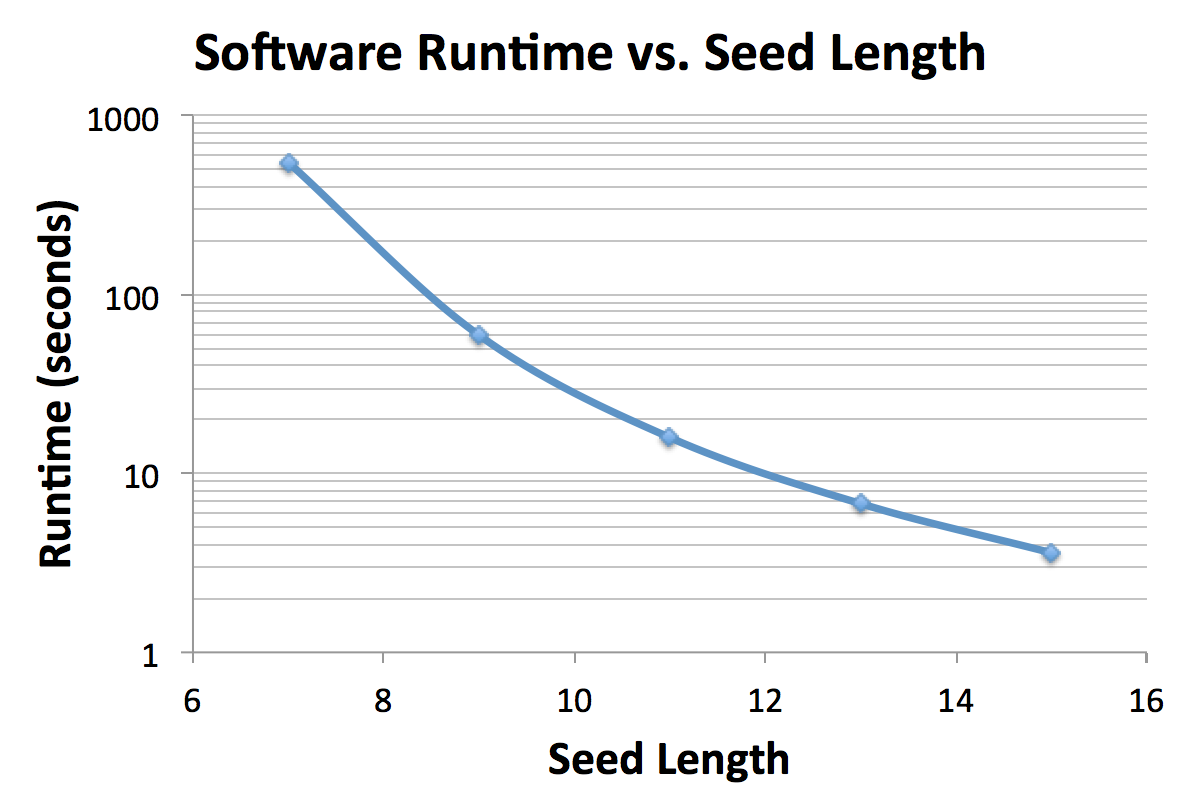
\includegraphics[width=90mm]{swruntime.png}
\caption{}
\label{speedvsseedlen}
\end{figure}

\begin{figure}[ht!]
\centering
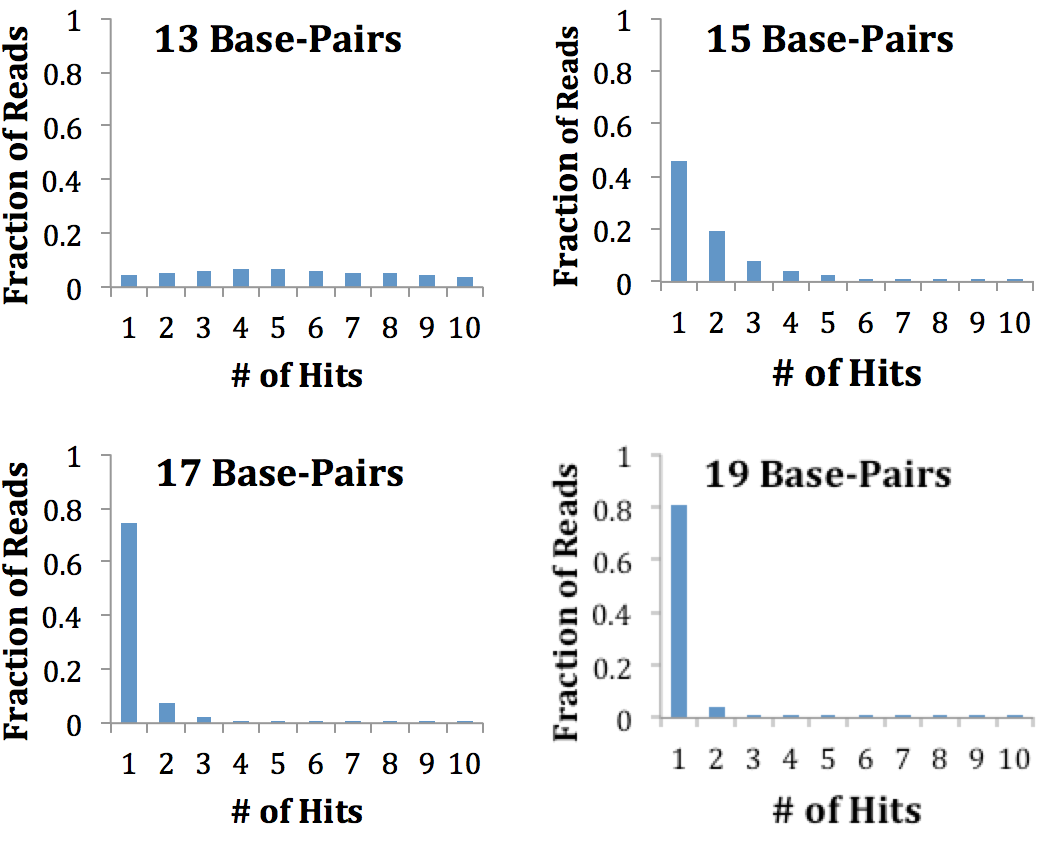
\includegraphics[width=90mm]{readsvhits.png}
\caption{Distribution of Hits as a Function of Number of Base Pairs}
\label{histogram}
\end{figure}


\section{Impact of Compression}
Understanding that the bottleneck for a hardware implementation is the memory bandwidth, we would like to improve the memory bandwidth utilization.  One way to do this is to compress the position table so that fewer memory accesses are required to read a subread's position list.  Note that the goal of the compression is to reduce the number of memory accesses to read a full list, not necessarily to minimize the absolute size of the table.  The compressed table must still be locally indexable given a seed.

Given that the list of positions for each seed are stored consecutively in ascending order, we can apply delta encoding to reduce the number of bits required to store each position.  An example compression scheme is as follows.  The first four bytes of a list store the first position in the list.  Each subsequent position is stored as the difference from the previous position.  Deltas are encoded with variable numbers of bytes, with the lower seven bits of a byte encoding delta data.  The MSB of each byte indicates if the byte is the last for the current delta.

We generate compressed position tables for the 225 million base pair human chromosome with seed lengths varying from 7 to 15.  Figure \ref{compratio} indicates a reasonable compression ratio for small seed lengths. However, as we increase the seed length, the benefit of compression dramatically diminishes.  This is intuitive, since the number of positions for each seed decreases as we increase the seed length, and sparse lists do not compress well with delta encoding.  Given that performance dramatically improves with increased seed length, we would like to have the longest seed possible, where compression produces very little benefit.  Therefore, we do not use compression in our final implementation.
\begin{figure}[ht!]
\centering
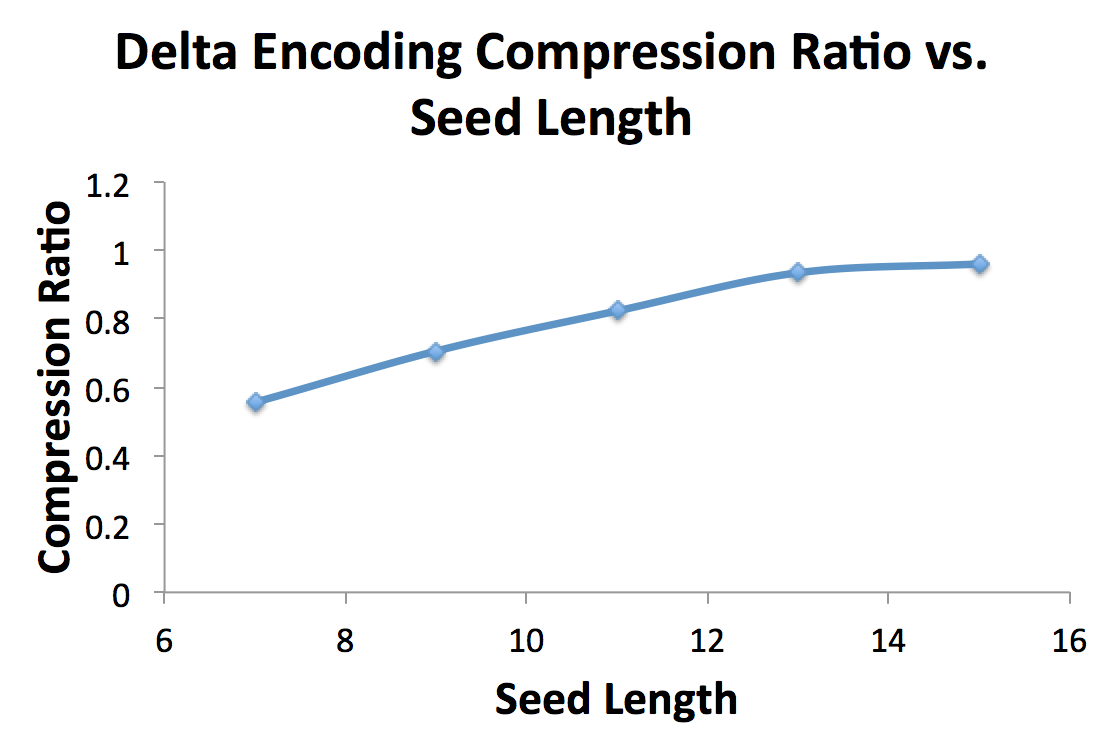
\includegraphics[width=90mm]{compratio.png}
\caption{}
\label{compratio}
\end{figure}


\section{Hardware Architecture}

The hardware architecture, as seen in Figure \ref{arch}, divides the sequencing operation into four main stages.  First, we have an Input Reader to fetch queries from memory.  This module subdivides the queries into shorter subreads before dispatching them to the Interval Table Controller (ITC).  Once they arrive at the ITC, the ITC uses the subread itself as the memory address, and fetches the start of the interval.  It fetches the end of the interval by looking at the immediate next position in memory.  This interval is then sent to the Position Table Controller (PTC), which requests all values in memory through the range of the interval.  Those values are then merged in the stitcher unit, which takes input from $N$ PTCs, $N$ being the number of subreads per input query.
\begin{figure}[ht!]
\centering
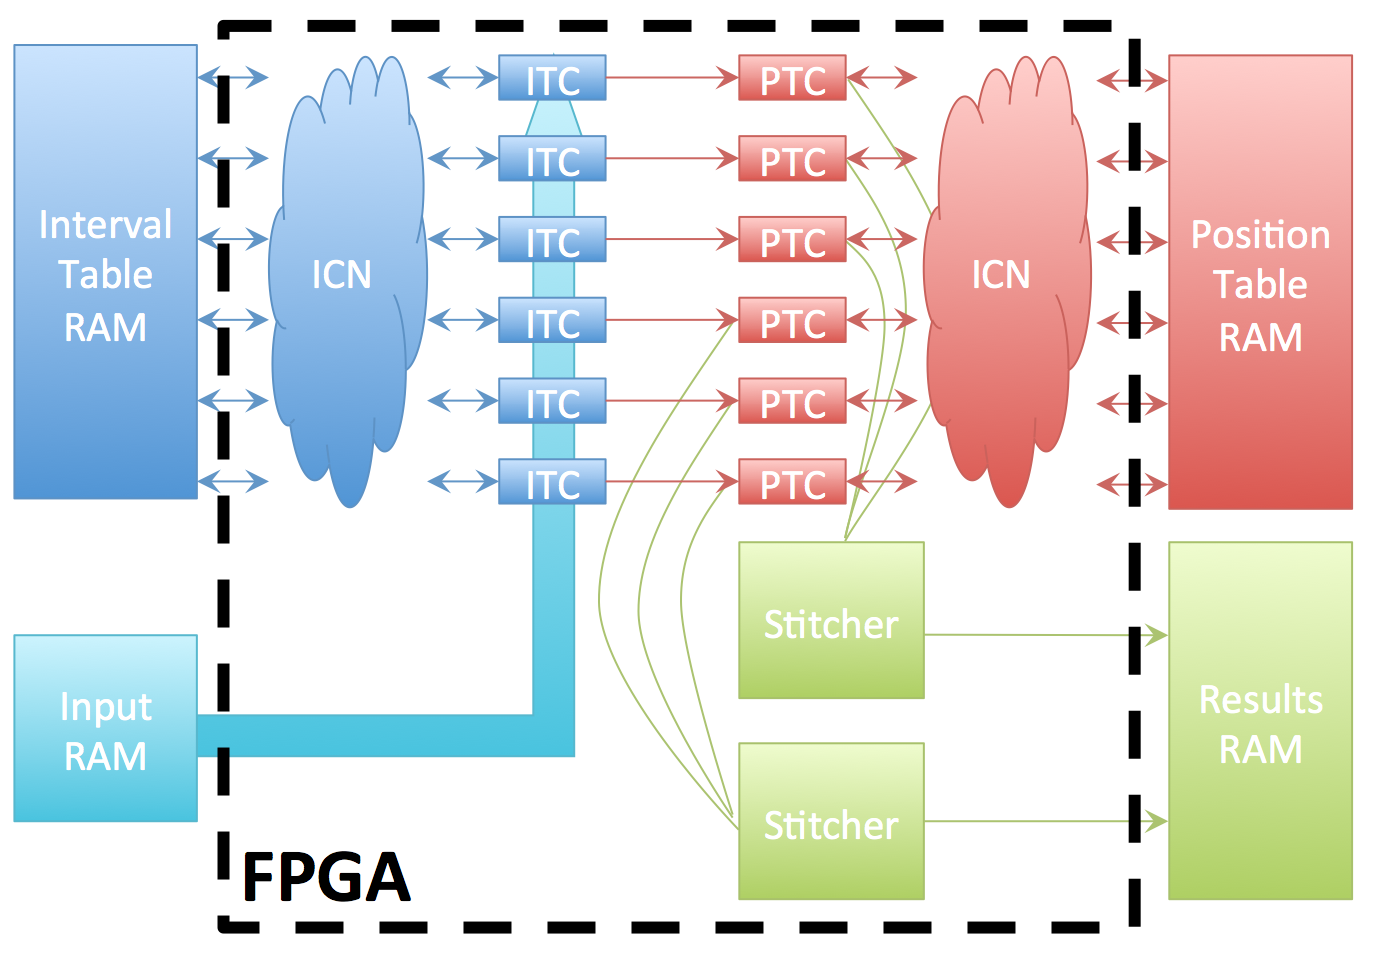
\includegraphics[width=90mm]{architecture.png}
\caption{Hardware Architecture}
\label{arch}
\end{figure}


\subsection{Memory System}
The hardware architecture includes three primary RAM systems - the input RAM to hold query sequences, the interval table RAM to hold the interval table, and the position table RAM to hold the position table.  Since the input is read sequentially and feeds multiple interval table controllers, we  stripe the data across all RAM chips and access them all in parallel.  For the tables, the memory system has to handle many concurrent accesses, so we developed a memory architecture that could multiplex multiple read ports to a number of individual RAM banks.  Since our access pattern for the ITC is entirely random and determined by the individual input subreads, optimizing our memory for reads substantially shorter than a standard cache line enables us to have other ports reading at the same time instead, provided two ports are not attempting to access the same RAM at the same time.


The PTC memory has a similar workload in that the initial address of each request can be anywhere in the memory.  Especially in cases of short subread lengths, however, it can require more than two reads to extract all the positions for a given subread.  As seen by our data from our software simulation, we favor a long subread length which means less entries in the PTC on average for a given subread.  To improve RAM bandwidth utilization, we also load data into our RAMs in a specific fashion.  By spreading the data evenly across all banks in the memory system, we maximize the potential bandwidth assuming a randomized set of read addresses (which is, in this case, largely correct).  Spreading evenly across RAM chips and their banks enables us to maximize bandwidth by pipelining requests to individual banks.

Since the design features multiple discrete memory chips, values requested from two different RAMs can return out of order.  Our solution, as seen in Figure \ref{rammodel}, is to place a reorder buffer in each read port, that is reserved upon read request and must retire in order.  The request information for each particular RAM is buffered alongside the RAM in a FIFO.  That provides enough information for us to route the output of the RAM to the reorder buffer of the correct port.  
\begin{figure}[ht!]
\centering
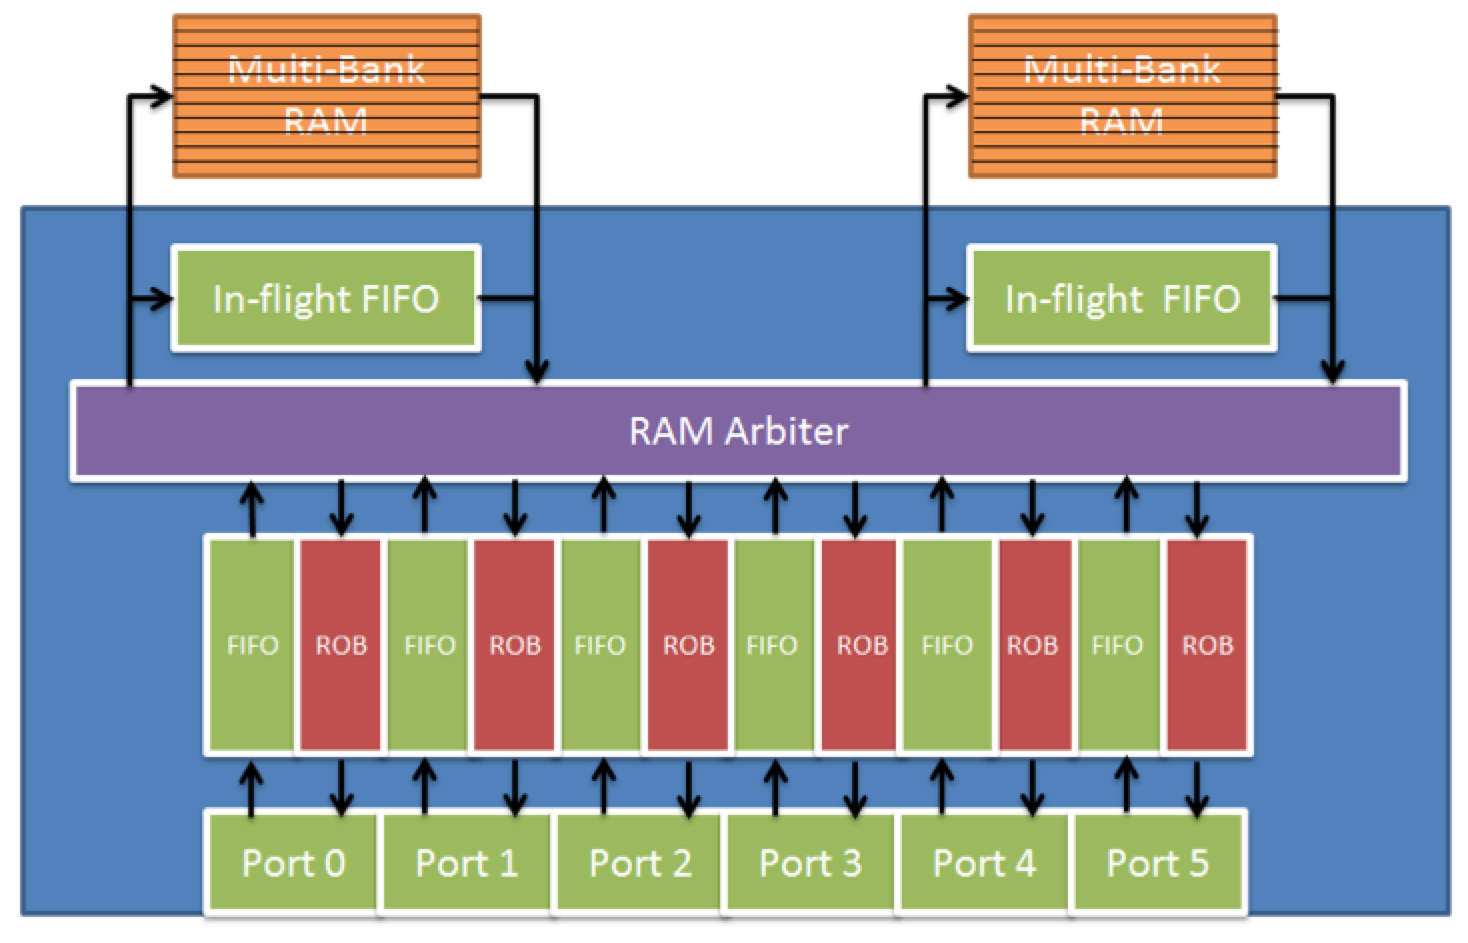
\includegraphics[width=90mm]{rammodel.png}
\caption{Memory System}
\label{rammodel}
\end{figure}

\subsection{Stitcher Operation}
The position results for a particular query are streamed, in ascending order, into the stitcher unit.  The stitcher unit has the same number of input ports as the number of subreads in a given query, each associated with a PTC.  Upon finishing its previous query, the stitcher waits for each PTC to provide a position to compare.  For each set of positions from the PTCs, it performs a matching operation.  If all of the positions match, then the result is stored.  If they do not, all but the highest positions are flushed from their respective queues.  The positions that are successfully stitched represent the offsets into the reference genome where a particular query can be found.

\subsection{Simulation and Performance}
To determine how our architecture performs, we performed a cycle-accurate simulation of the entire system, including RAM timings, that allow us to analyze performance as we vary the memory size and processing resources (stitchers and associated ITCs and PTCs).  The results, as seen in Figure \ref{utilization}, show that despite our large improvements to memory utilization beyond conventional systems, we are still memory bandwidth bound assuming a realistic memory system model.  
\begin{figure}[ht!]
\centering
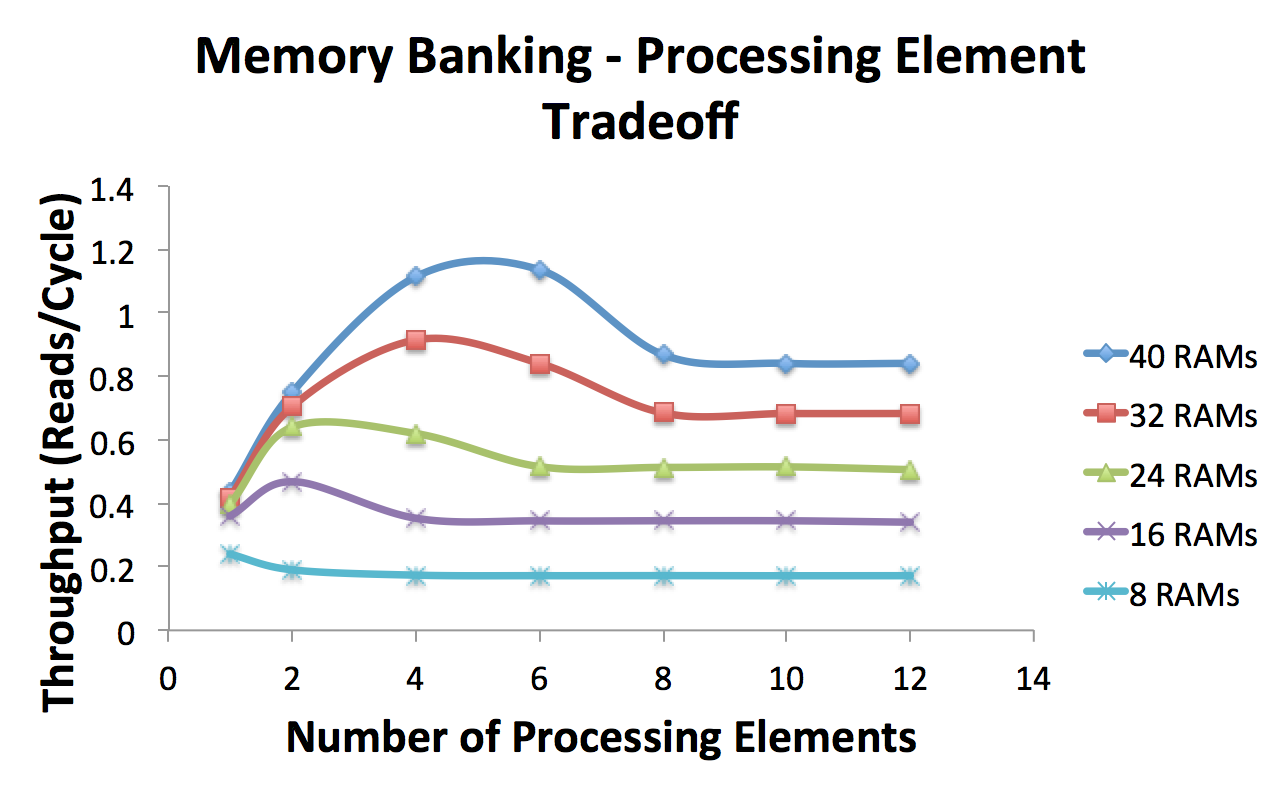
\includegraphics[width=90mm]{memproc.png}
\caption{}
\label{utilization}
\end{figure}

The results of our simulation indicate that the addition of processing elements has the potential to decrease performance after a certain point.  We compare throughput of the system with the number of stitching units, varying from 1 to 12, with a variety of memory configurations.  In every single case, as we add stitchers past the maximum, the performance degrades.  This is because of additional contention in the memory system as we are already extracting the maximum bandwidth from the memory with fewer processing elements.  A potential way to resolve this issue is to allow out-of-order memory accesses, prioritized by the availability of each RAM chip in the system.  

\section{Analytical Model}
 
To estimate the relationship between the number of ITCs, PTCs, stitchers, and RAMs, we developed a first order approximation to determine the amount of contention seen by the ITCs and PTCs when accessing the interval table and position table RAMs, respectively. Given our pipelining structure, the number of ITCs and PTCs were each the same, with there being one stitcher for every $m$ ITCs and PTCs, $m$ being the number of subreads per query. Essentially, as a rough approximation, full memory bandwidth is achieved when each ITC or PTC accesses a different memory bank each clock cycle - giving us the most parallel accesses to the memory.
 
Thus, to estimate the bandwidth utilization we can calculate the expected number of memory banks hit per clock cycle, given $B$ total banks and $N$ controllers trying to access them. To do this, define $I_b$ to be the indicator variable for whether bank $b$ was hit by any of the $N$ controllers. Then
\begin{eqnarray*}
H&=&\frac{1}{B}E\left(\sum_{b=1}^{B} I_b\right)
\end{eqnarray*}
where $H$ is the expected bandwidth utilization. Following this train of thought, we see:
\begin{eqnarray*}
H&=&\frac{1}{B} \sum_{b=1}^{B} E(I_b) \\
H&=&\frac{1}{B} \sum_{b=1}^{B} P(I_b = 1) \\
H&=&\frac{1}{B} \sum_{b=1}^{B} \left(1-\left(\frac{B-1}{B}\right)^N\right) \\
H&=& 1-\left(\frac{B-1}{B}\right)^N
\end{eqnarray*}
Thus, for a given $H$ we can solve for $N$:
\begin{eqnarray*}
N&=&\frac{\log{(1-H)}}{\log{(B-1)}-\log{B}}
\end{eqnarray*}
Note that this is a first order approximation - if we were to have too many controllers accessing $B$ banks, then there will be backlog at the banks and bandwidth starts to be adversely affected. As a rule of thumb, we saw that setting $H$ close to 85\% kept us from seeing these second order effects. Plotting this for a large range of $B$ shows this can be simplified to saying $N \approx 1.8B$. This provides a good design heuristic for finding a starting point when configuring the hardware system.

\section{Conclusions}

Modern genomic research has paved the way towards personalized medicine, where medical care can be specifically tailored to the individual based on his or her genome.  Combined with the rapid decline in sequencing costs, the demand for individual whole genome sequencing is expected to rise in the near future.  Short read alignment, the computational bottleneck of the sequencing process, has been a focus of research for decades to improve accuracy and performance.  It is becoming evident that novel hardware acceleration techniques will be necessary to achieve the required throughput to keep up with demand in a cost effective manner.


	We explored an example exact alignment algorithm that divides a short read into seeds. We perform table lookups to identify the list of reference sequence positions that each seed maps to, and then stitch together the position lists of the seeds to produce the list of hits for the full read.  This is a commonly used technique in inexact alignment algorithms to improve performance, as in \cite{ning2001ssaha, toh2009basic, zaharia2011faster}.  Our study shows the benefits of increasing the seed length to improve performance, due to the reduced position list lengths of the seeds.


We designed a hardware architecture to accelerate this algorithm that utilizes a parallel multi-chip memory architecture to increase the random access memory bandwidth.  We built a cycle-accurate simulator to verify the model, and to explore the bottlenecks and tradeoffs of the architecture.  We saw that the architecture is almost entirely memory bandwidth limited, showing that increasing the number of processing elements beyond a certain threshold no longer affects performance, while increasing the number of parallel RAM chips continues to improve performance linearly.  We therefore conclude that cost effective performance hinges upon improving memory bandwidth, rather than increasing pure compute power.

\section{Future Work}

We showed that the performance of our algorithm improves with increased seed length.  However, our implementation currently does a table lookup using the seed itself, and increasing the seed length increases the table size exponentially to infeasibility.  To reduce the memory requirement at the cost of more lookups, we can store the seeds into a hash table.  However, this would provide a worst case performance for inexact alignment, where not all seeds are guaranteed hits, since a lookup would require a traversal through an entire bin before recognizing that there are no hits.  Different hash table organizations and hashing functions can be explored to improve performance.


Given that this study was only a case study for a particular exact alignment algorithm, we would like to explore various inexact alignment algorithms in the future.  Of particular interest is the family of algorithms using the Burrows Wheeler Transform \cite{li2009fast}.  We expect the performance to be even more memory bandwidth limited, since the BWT based algorithms almost purely involve memory lookups with very little computation.


Finally, we would like to implement the architecture on an FPGA with a custom memory system to validate our results, and to provide a high performance, cost effective tool for the bioinformatics community to expedite their research.




\bibliographystyle{latex8}
{
  % If you have space problems...
  %\setstretch{1.0}
  \bibliography{cs316_paper}
}


\end{document}
